\begin{center}
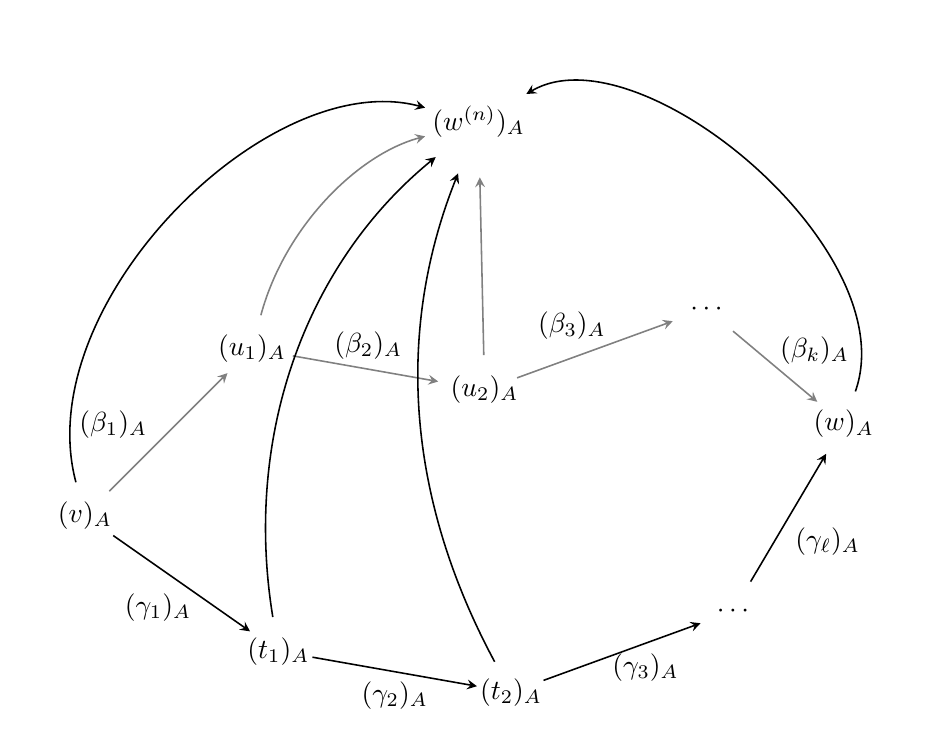
\begin{tikzpicture}[line width = 0.2mm, >=stealth, shorten >= 12.5pt, shorten <=12.5pt]
\draw[->, Black!50!White] (0,0) coordinate (a1)
-- node[above, xshift = -0.7cm, yshift = -0.2cm] {$\textcolor{Black}{(\beta_1)_A}$}
++(45:3) coordinate (a2);
\draw[->, shorten >= 17pt, shorten <=15pt, Black!50!White] (a2)
-- node[above] {$\textcolor{Black}{(\beta_2)_A}$}
++(-10:3) coordinate (a3);
\draw[->, Black!50!White, shorten >= 13pt] (a3)
-- node[above, xshift = -0.3cm] {$\textcolor{Black}{(\beta_3)_A}$}
++(20:3) coordinate (a4);
\draw[->, Black!50!White] (a4)
-- node[above, xshift = 0.5cm, yshift = -0.1cm] {$\textcolor{Black}{(\beta_k)_A}$}
++(-40:2.275) coordinate (a5);
\node at (a1) {$(v)_A$};
\node at (a2) {$(u_1)_A$};
\node at (a3) {$(u_2)_A$};
\node at (a4) {$\cdots$};
\node at (a5) {$(w)_A$};

\draw[->] (0,0)
-- node[below, xshift = -0.3cm] {$(\gamma_1)_A$}
++(-35:3) coordinate (a6);
\draw[->] (a6)
-- node[below] {$(\gamma_2)_A$}
++(-10:3) coordinate (a7);
\draw[->, shorten >= 12.5pt] (a7)
-- node[below, xshift = 0.3cm, yshift = 0.1cm] {$(\gamma_3)_A$}
++(20:3) coordinate (a8);
\draw[->] (a8)
-- node[below, xshift = 0.5cm] {$(\gamma_{\ell})_A$}
(a5);
\node at (a6) {$(t_1)_A$};
\node at (a7) {$(t_2)_A$};
\node at (a8) {$\cdots$};
\coordinate (a9) at (5,5);
\node at (a9) {$(w^{(n)})_A$};
\foreach \n/\ang/\col in {1/60/{Black},2/30/{Black!50!White}, 3/0/{Black!50!White}, 5/-70/{Black}, 6/30/{Black}, 7/25/{Black}}{
\draw[->, \col, shorten >= 20pt] (a\n) to[bend left = \ang] (a9);
}
\end{tikzpicture}
\end{center}